
\section{Image Compression}
\label{sec:img}

As indicated in section~\ref{sec:intro} we would like to use the wavelets for compression. If the image is appropriately transformed to the wavelet domain we can throw away coefficients with a small absolute value. These values influence the image only subtely. In this section we will investigate the possibilities of using this method for compression and look at the different difficulties. We will restrict ourselves to gray images.

\subsection{Compression}
In this subsection we will consider an image $X$ to be a real valued $n \times m$-matrix: $X = \{x_{i,j} \| 0 \leq i \leq n,\, 0 \leq j \leq m\}$ (again $n$ and $m$ are powers of two). To determine the compression rate we have to make some assumptions on sizes of certain types. We assume a real value to be 8 bytes, and an index to be 4 bytes. This assumption restricts the size of the matrix ($0 \leq n < 2^32$ and $0 \leq m < 2^32$). Thus the original image $X$ has a size of $8 \times mn$ bytes, as we can store the matrix as an contiguous array (we ignore the fact that we should also store the size). As discussed in section~\ref{sec:dau} we can apply the Daubechies wavelet transform in both directions, which results in a matrix $Y = \{y_{i,j} \| 0 \leq i \leq n,\, 0 \leq j \leq m\}$ (again of the same size). The idea is to throw away all element $y_{i,j}$ with $|y_{i,j}| \leq \tau$ for some threshold parameter $\tau$. The result is the compressed image:
\[ C = \{ (y_{i,j}, i, j) \| 0 \leq i \leq n, 0 \leq j \leq m, |y_{i,j}| \leq \tau \}. \]
Note that we now have to store the location of the coefficients bigger than the threshold $\tau$. Assume that we did not throw away $c$ of the $nm$ coefficients. Then the compressed size is $(8+4+4) \times c = 16 \times c$. So this compression becomes useful when $c \leq \frac{1}{2}nm$. This might seem like a big loss in quality. But as we can see in figure~\ref{fig:compression}, the wavelets are capable of capturing the important shapes and edges of the image.


\begin{figure}
	\begin{subfigure}[b]{0.25\textwidth}
		\centering
		\includegraphics[width=\textwidth]{oostenrijk.png}
		\caption{Original}
	\end{subfigure}~
	\begin{subfigure}[b]{0.25\textwidth}
		\centering
		\includegraphics[width=\textwidth]{10oostenrijk.png}
		\caption{$\rho=\frac{1}{10}$}
	\end{subfigure}~
	\begin{subfigure}[b]{0.25\textwidth}
		\centering
		\includegraphics[width=\textwidth]{100oostenrijk.png}
		\caption{$\rho=\frac{1}{100}$}
	\end{subfigure}~
	\begin{subfigure}[b]{0.25\textwidth}
		\centering
		\includegraphics[width=\textwidth]{1000oostenrijk.png}
		\caption{$\rho=\frac{1}{1000}$}
	\end{subfigure}
	\caption{Test image with a fraction $\rho$ of the coefficients left.}
	\label{fig:compression}
\end{figure}

As the wavelet transform is invertible we can decompress $C$ to obtain a approximation of $X$.


\subsection{Practical difficulties}
We made a big assumption in the previous subsection which does not hold at all in the real world. Namely that an image $X$ is a \emph{real valued} $n \times m$-matrix. Most images are quantized to take values in $[0, 255]$, i.e. images consists of pixels of a single byte. This means that the size of an image $X$ is simply $nm$ bytes. Our algorithm only works for real valued data, so we can convert these bytes to the reals and perform our algorithm to obtain $Y$. The values of $X$ are nicely distributed in $[0, 255]$, whereas $Y$ has a totally different distribution, most of it is concentrated around 0. This blow-up from 1 byte to 8 bytes is still to big, so we would like to quantize the values which we do not throw away. For a suitable quantization $f: \R -> [0, 255]$ the compressed image is now:
\[ C = \{ (f(y_{i,j}), i, j) \,|\, 0 \leq i \leq n, 0 \leq j \leq m, |y_{i,j}| \leq \tau \}, \]
with a size of $9c$ instead of $mn$. In figure~\ref{fig:comrpession_algo} the different steps of the algorithm are depicted.

The only thing left is to specify the quantization function $f$. We want it to have three properties. First of all we would like it to be invertible in order to decompress the image. Of course this is impossible, but we can ask for a function $g$ such that $|y - g(f(y))|$ is somewhat minimized. Secondly, we want $f$ to make the distribution of $Y$ more uniform. And at last we do not want $f$ to account the values we will throw away. In figure~\ref{fig:quantization} three such functions are considered. For the exact details we refer to the implementation. Note that a linear quantization performs very bad.

\begin{figure}
	\begin{subfigure}[b]{0.25\textwidth}
		\centering
		\includegraphics[width=\textwidth]{eindhoven.png}
		\caption{Original}
	\end{subfigure}~
	\begin{subfigure}[b]{0.25\textwidth}
		\centering
		\includegraphics[width=\textwidth]{eindhoven_lin.png}
		\caption{Linear}
	\end{subfigure}~
	\begin{subfigure}[b]{0.25\textwidth}
		\centering
		\includegraphics[width=\textwidth]{eindhoven_log.png}
		\caption{Logarithmic}
	\end{subfigure}~
	\begin{subfigure}[b]{0.25\textwidth}
		\centering
		\includegraphics[width=\textwidth]{eindhoven_sqrt.png}
		\caption{Square root}
	\end{subfigure}
	\caption{Three different methods to quantize the coefficients.}
	\label{fig:quantization}
\end{figure}


\subsection{Parallel implementation}
We have already seen how to perform a two-dimensional wavelet transform in section~\ref{sec:dau}. By parallelizing the one-dimensional case we get one for two dimensions for free. However, we can do a bit better. There was a slight problem in the parallelization, namely that there was a dedicated processor which had to end the algorithm. With more data at hand we can now do this last step too in parallel. Let $X$ be an image of width $w$ and height $h$ and let $p$ be the number of processors. We divide the image into blocks of size $\frac{w}{p}\times\frac{h}{p}$. We will assign processors to these blocks as shown in figure~\ref{fig:par2d}. When doing the wavelet horizontally we will let processor 0 finish the first $\frac{w}{p}$ rows, processor 1 the second $\frac{w}{p}$ rows, and so on. Similarly for the columns. This assignment ensures that all processors will end the algorithm for some rows and columns, hence no processors will be idling.

\begin{figure}
	\centering
	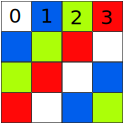
\includegraphics{2dpar}
	\caption{Assignment of blocks to processors 0, 1, 2 and 3}
	\label{fig:par2d}
\end{figure}

The sequential cost of the algorithm is $28wh$, as we have to perform the wavelet in both directions. Most part of the analysis of the previous section still holds. Let us consider doing the wavelet horizontally for each row, instead of sending $C_m$ words in each step, we now have to send $\frac{h}{p}C_m$ words and so on. Almost every term in the cost analysis is multiplied by $\frac{h}{p}$, except for the factors of $l$, as we do not have to synchronize more often (we only have to send bigger chunks of data). Doing this in both directions yields the cost of the parallel two-dimensional wavelet transform:
\begin{align*}
	T &= 14\frac{h}{p}D_m^H + 14\frac{h}{p}p + \frac{1}{m}\logt(\frac{w}{p})(\frac{h}{p}C_m^Hg+l) + 2(p-1)\frac{h}{p}g + 2l \quad\text{ (horizontal part)}\\
	  &+ 14\frac{w}{p}D_m^V + 14\frac{w}{p}p + \frac{1}{m}\logt(\frac{h}{p})(\frac{w}{p}C_m^Vg+l) + 2(p-1)\frac{w}{p}g + 2l \quad\text{ (vertical part)}
\end{align*}
In particular, if $n=w=h$ and $m=1$, we can simplify this to:
\[ T = 28\frac{n^2}{p} + 28n + 2\logt(\frac{n}{p})(2\frac{n}{p}g+l) + 4(p-1)\frac{n}{p}g + 4l \text{ flops}, \]
compared to the $28n^2$ flops of the sequential algorithm.

